\documentclass{school-22.211-notes}
\date{February 22, 2012}

\begin{document}
\maketitle

\subtopic{Spectral Code} 
Review slides. 

\topic{Temperature Effects on Cross Section (Doppler Broadening)}
\subtopic{Resonance Integrals}
We introduce \hi{Resonance Integrals} as flux weighted (that is, weight with 1/E spectrum in our case so far because $\phi(E) = \frac{1}{E}$) micro-scopic cross section:
\eqn{ \mathrm{RI} = \frac{\int_{E_1}^{E_2} \sigma_{238} (E) \phi(E) \dE}{\int_{E_1}^{E_2} \phi (E) \dE }  }

As the \hi{Dilution Factor (U/H)} goes to zero, we get infinite dilution, which is what we have been modeling so far. Infinite dilution factor is about 10 or 20 times bigger than a real dilute in a LWR. As the dilution factor increases and approaches a real case, the U238 increases, we would observe more dips in the flux vs. lethargy plot from U238's resonance xs as seen in Figure~\ref{dilution-factor-increase}. 
\begin{figure}
  \centering
  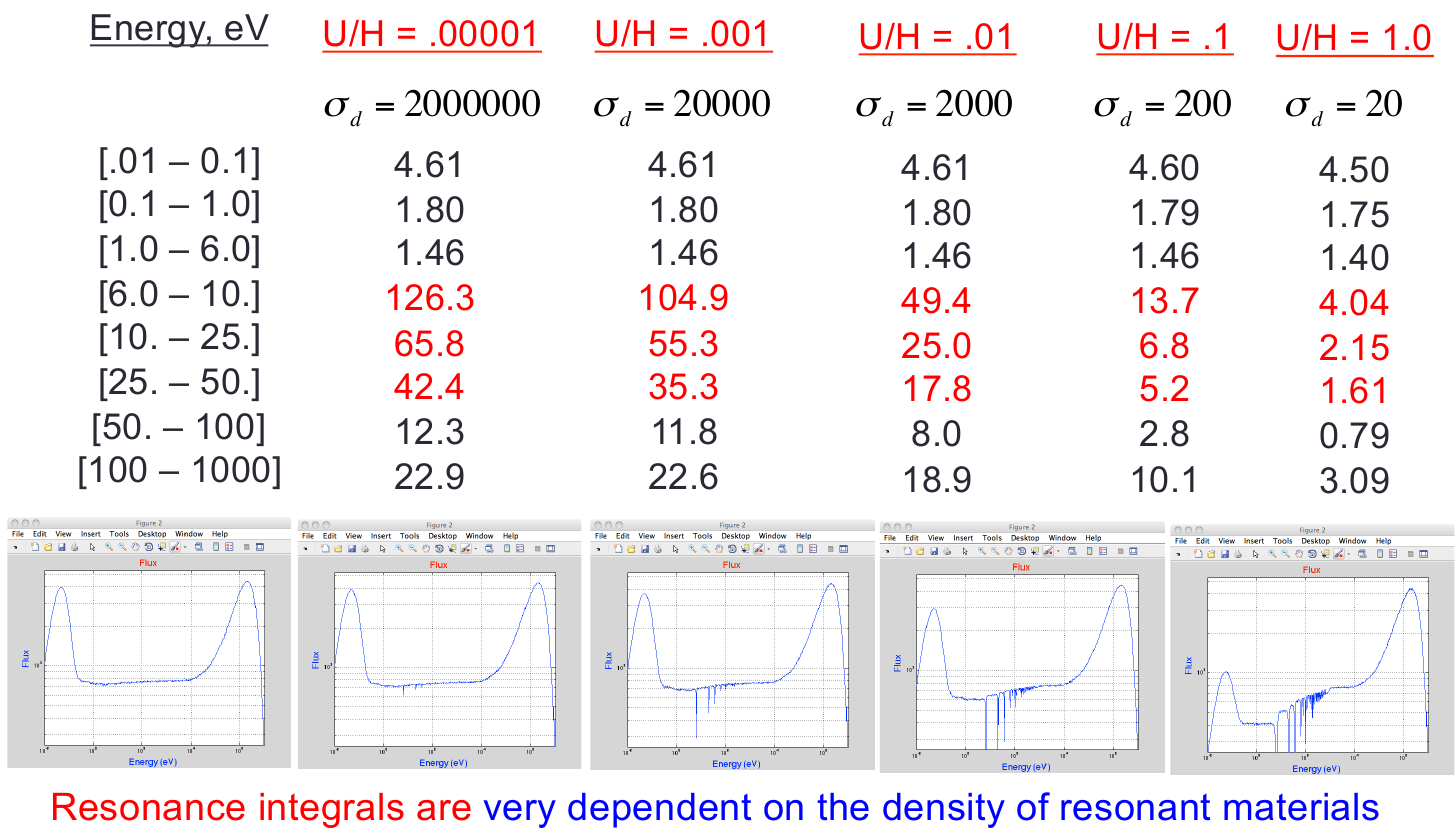
\includegraphics[width=2in]{images/dilution-factor-increase.png}
  \caption{Resonance Dips Increase As U/H Increases} \label{dilution-factor-increase}
\end{figure}

\subtopic{Doppler Broadening}
Resonance Integrals increase with increasing temperature. \hi{Doppler Broadening} means, if the width of the spectrum decreases, because the area under the curve stays the same, the depth of the resonance trap would increase and approach infinity eventually, but the probability of neutron slowing down would decrease. 

In general, doppler broadening is the broadening of spectral lines due to the Doppler effect caused by a distribution of velocities of atoms or molecules. There are a couple of different kinds of Doppler broadening, including the thermal Doppler broadening due to the thermal motion of the particles; also, there are broadening depends on the frequency of the spectral line, the mass of the emitting particles, and the temperatures. 

Reference 1: Reuss Section 8.4. 

Reference 2: Handbook of Nuclear Engineering Chapter 4 Section 3. 

\end{document}
